\DeclareGraphicsExtensions{.pdf,.png,.jpg}

\chapter{Конструкторский раздел}
\label{cha:design}

В данном разделе будет произведена конкретизация задач и проанализированы алгоритм.

\section{IDEF0 Модель}

На рисунке 2.1 приведена функциональная модель шифрования в нотации IDEF0.
\begin{figure}[H]
\centering
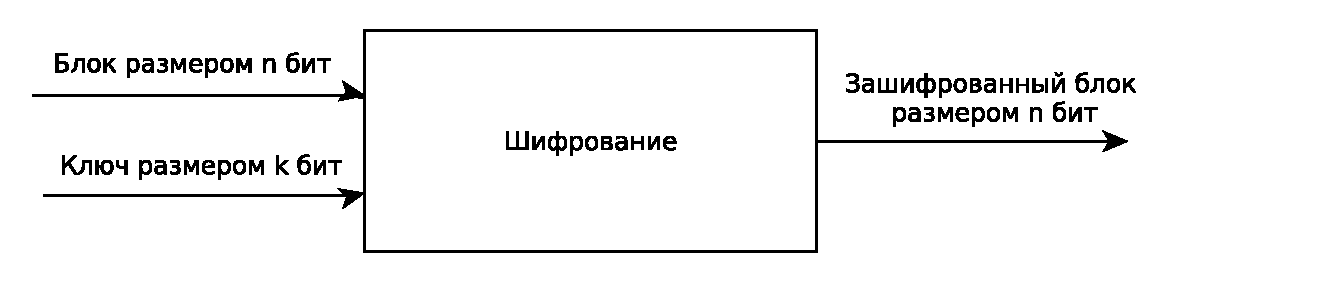
\includegraphics[scale=0.75]{./pict/ideftr.pdf}
\caption{Функциональная модель шифрования}
\end{figure}
\newpage

\section{Разработка алгоритмов}
Подробная схема шифрования алгоритма DES представленна на рисунке 2.2.

\begin{figure}[H]
\centering
\includegraphics[scale=1.2]{./pict/Code.png}
\caption{Алгоритм DES}
\end{figure}

\section{Вывод}
В данном разделе была рассмотрена схема алгоритма.
